\lecture{07.11.2023}

\begin{lem}
	Let \( K \) be a number field as above.
	Then there exists a \( \Q \)-basis of the number field, say \( (\alpha_1, \dotsc, \alpha_n) \), with \( \alpha_1, \dotsc, \alpha_n \in \Ocal_K \).
\end{lem}

\begin{prop}\label{thm:1.22}
	Let \( (\alpha_1, \dotsc, \alpha_n) \) be a \( \Q \)-basis of a number field \( K \) with \( \alpha_1, \dotsc, \alpha_n \in \Ocal_K \), \( d = \disc(\alpha_1, \dotsc, \alpha_n) \) and \( \beta \in \Ocal_K \).
	Then there exist \( m_1, \dotsc, m_n \in \Z \), such that
	\[ \beta = \frac{m_1\alpha_1 + \dots + m_n\alpha_n}{d} \]
	and \( d \divides m_i^2 \) for \( 1 \leq i \leq n \).
\end{prop}

\begin{lem}
	Let \( K \) be a number field with integral bases \( (\alpha_1, \dotsc, \alpha_n) \) and \( (\beta_1, \dotsc, \beta_n) \).
	Then
	\[ \disc(\alpha_1, \dotsc, \alpha_n) = \disc(\beta_1, \dotsc, \beta_n). \]
\end{lem}

\begin{defn*}[Discriminant of \( K \)]\index{Discriminant}
	Let \( K \) be a number field and \( (\alpha_1, \dotsc, \alpha_n) \) a \( \Z \)-basis for \( \Ocal_K \).
	We define the \emph{discriminant} \( \disc(K) \) of \( K \) as
	\[ \disc(K) = \disc(\alpha_1, \dotsc, \alpha_n). \]
\end{defn*}

\begin{exmp*}
	Let \( d \in \Z \) be squarefree. Then
	\[ \disc\big(\big[\sqrt{d}\big]\big) = \begin{cases}
		4d &d \equiv 2,3 \mod 4,\\
		d &d \equiv 1 \mod 4.
	\end{cases} \]
\end{exmp*}


\section{Cyclotomic fields}

\begin{wrapfigure}{R}{2cm}
	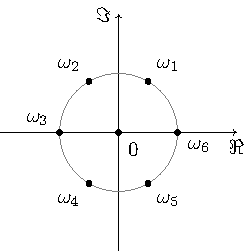
\includegraphics{sixth_roots}
\end{wrapfigure}

\begin{defn*}
	For \( m \in \N \) we call \( \Q \left[ e^\frac{2\pi i}{m} \right] \) the \( m \)-th cyclotomic field.
\end{defn*}

%\begin{minipage}{\linewidth}
%	\begin{wrapfigure}{R}{2cm}
%		\centering
%		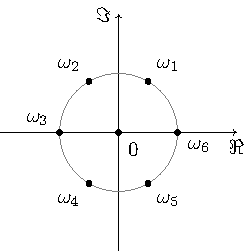
\includegraphics{sixth_roots}
%	\end{wrapfigure}
	\begin{exmp*}
		\begin{itemize}
			\item The first two cyclotomic fields are equal to \( \Q \).
			\item Let \( m = 6 \) and write \( \omega = e^\frac{2\pi i}{6} \).
		Then \( \omega^5 = -\omega^2 \), i.e. \( \omega = -\omega^4 \) and \( \Q[\omega] = \Q[\omega^2] \).
		This means that the third and sixth cyclotomic fields are equal.
		
		\end{itemize}
	\end{exmp*}
%\end{minipage}
			

In the following let \( m \in \N \) and write \( \omega = e^\frac{2\pi i}{m} \).

\begin{thmn}
	The extension \( \Q[\omega] \) over \( \Q \) is Galois with degree equal to \( \varphi(m) \), where \( \varphi \) is Euler's totient function.
	Moreover, the Galois group is isomorphic to \( (\Z/m\Z)^* = \set{k \in \Z/m\Z}{\gcd(k,m)=1} \).
\end{thmn}

For \( k \in (\Z/m\Z)^* \) the corresponding automorphism is given by \( \omega \mapsto \omega^k \).

\begin{prop}
	The conjugates of \( \omega \) are exactly given by \( \omega^k \) with \( \gcd(m,k)=1 \).
\end{prop}

\begin{cor}
	Let \( m \in \N \) be even.
	Then the roots of unity contained in \( \Q(e^\frac{2\pi i}{m}) \) are exactly the \( m \)-th roots of unity.
\end{cor}

\begin{cor}
	The \( m \)-th cyclotomic fields, for \( m \) even, are all non-isomorphic.
\end{cor}

\begin{thmn}
	Let \( m=p^r \) for some prime \( p \) and \( \omega = e^\frac{2\pi i}{m} \).
	Then \( \Ocal_{Q[\omega]} = \Z[\omega] \).
\end{thmn}

\begin{rem*}
More generally, \( Z[\omega] = \Ocal_{Q[\omega]} \) for \emph{every} cyclotomic field.
\end{rem*}

\begin{notat*}
	We write \( \disc(\alpha) = \disc(1, \alpha, \dotsc, \alpha^{n-1}) \).
\end{notat*}

\begin{lem}
	For \( m \in \N \) we have \( \disc(\omega) \divides m^{\varphi(m)} \).
\end{lem}